\textbf{(a) If two points are selected at random on the circumference of a circle of
radius $\rho$, use Monte Carlo simulation to estimate the probability that the distance between the points is greater than $\rho$.\\\\}

\begin{lstlisting}[style=CStyle]
/**
 * Homework 2.4
 * EECE 5643 - Simulation and Performance Evaluation
 * Author: Harrison Sun
 * Email: sun.har@northeastern.edu
 */

#define defaultradius		1.0
#define defaultseed			0L
#define numruns				100000

#include <iostream>
#include <math.h>
#include <stdlib.h>
#include "c_lib/rng.h"

/**
 * int main()
 * 
 * @param int argc - the number of arguments
 * @param char* argv[] - the array of arguments
 * 
 * This is the main function. It randomly selects two points on the circumference of a circle and calculates the distance between them. 
 * This program calculates the probability that this distance is greater than the radius.
 */

int main(int argc, char* argv[])
{
	long seed = (argc > 1) ? atol(argv[1]) : defaultseed;
	double radius = (argc > 2) ? atof(argv[2]) : defaultradius;

	PutSeed(seed);
	
	int count{ 0 };
	
	for (int i = 0; i < numruns; ++i)
	{
		/* Find the angle of the point on the circle. */
		double angle1 = 2 * M_PI * Random();
		double angle2 = 2 * M_PI * Random();
		
		/* Distance Formula */
		double distance = sqrt(pow((radius * cos(angle1) - radius * cos(angle2)),2) + pow((radius * sin(angle1) - radius * sin(angle2)),2));
		count += (distance > radius) ? 1 : 0;
	}
	
	std::cout << "The probability that the distance between two points on the circumference of a circle is greater than the radius is "
		<< (double)count / numruns << std::endl;
	
	return 0;
}
\end{lstlisting}
\newpage \noindent
Terminal Outputs:\\
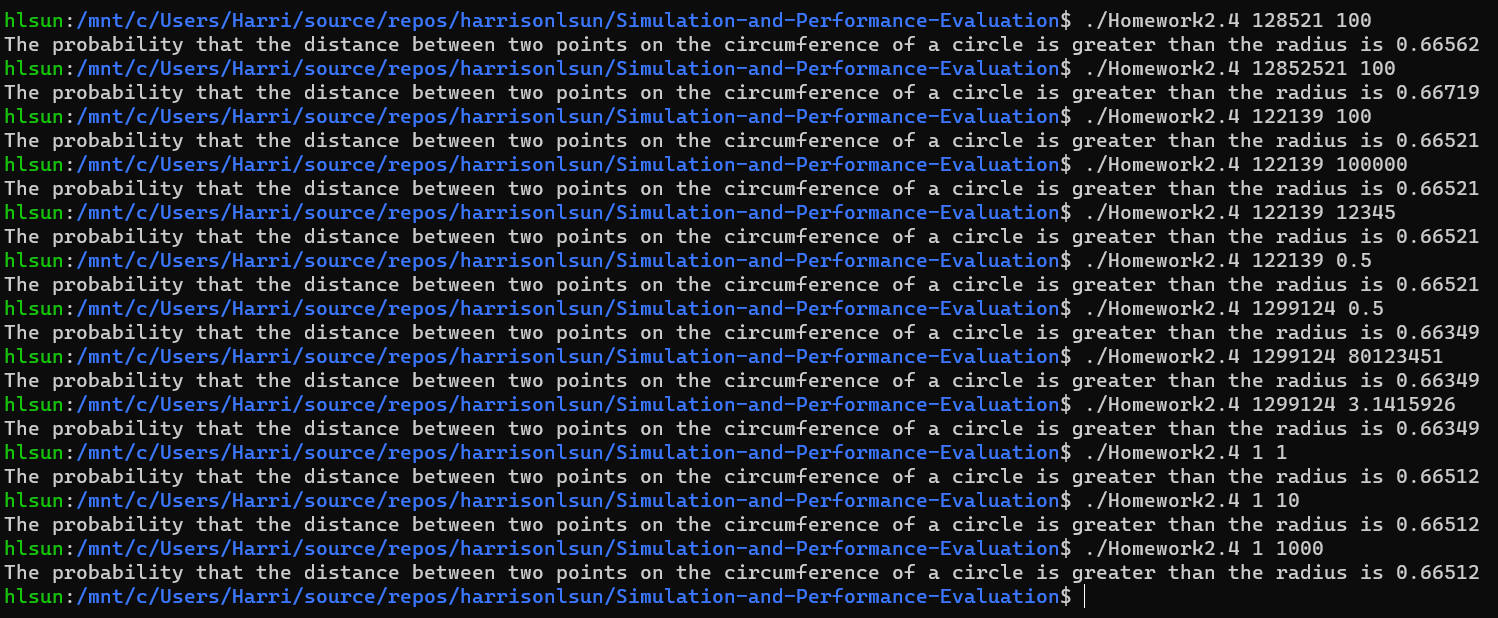
\includegraphics[scale=0.5]{Sections/H2_4.png}\\\\\\
